\chapter{Designing the driving scenarios} \label{chap:five}
This chapter explores various approaches for generating scenarios, with a specific focus on the method selected by this article. In \autoref{sect-5.1}, we start by giving an overview of some of the possible ways that scenarios could be generated, while \autoref{sect-5.2} and \autoref{sect-5.3} examine the chosen scenario and path generation methods and discuss their benefits and drawbacks in terms of accurately predicting new scenarios. Finally, in \autoref{sect-5.4}, we conclude the chapter by discussing potential improvements for the current method of scenario generation.

\section{How the driving scenarios could be designed} \label{sect-5.1}
Let us begin by discussing the need to design driving scenarios for autonomous vehicles. According to Ruxin Li and Runping Zhain's article ``Estimation and Analysis of Minimum Traveling Distance in Self-driving Vehicle to Prove Their Safety on Road Test" \cite{li2019estimation}, self-driving vehicles must drive at least 7.2 billion kilometres to prove their accuracy and confidence to an acceptable level. However, this distance is enormous, equivalent to circling the Earth approximately 180,000 times. If we imagine a car driving on the road 24/7 at an average speed of 60km/h, it would take that car 13,699 years to complete this distance. Therefore, simply putting a vehicle on the road and testing it to the fullest extent would be inadequate, given the time required. This is where the simulated environment comes into play.

A well-constructed framework that can accurately test how the software system controlling the autonomous vehicle behaves can be a huge time-saver allowing fully autonomous cars to see the daylight more quickly. However, as we will soon see, this task is very challenging, and some traditional ways of solving it might not work.

One of the traditional ways a scenario generation could be imagined is by designing the scenarios manually, putting objects into specific locations, and trying to recreate complex driving situations in the simulated world. However, time is the enemy, and doing everything by hand would not be much better than letting the autonomous vehicle drive for decades or even more. In addition, it is impossible to think of all the possible edge cases the vehicle might encounter because life is stochastic and non-fully observable. An infinite amount of possible things can happen at any given time, and hard-coding them in the software would bring poor yield. What is needed is a way of creating complex and realistic driving situations automatically, and assessing how good the generated scenarios are.

This is a perfect moment to start talking about AI in a bit more depth and discuss how it can help us in the case of scenario generation. Specifically, the rest of this section focuses on machine learning, a concept that has long been laid on the shelf and was made possible in practice only in the last few decades because of the immensely increased computational power resources and advanced hardware capabilities. Although a young member of the technology field, machine learning has already demonstrated its significance in various areas, such as medicine for predicting illnesses, economics and finance for predicting market changes, etc.

One of the fascinating aspects of machine learning applications is that they are not ordinary programs designed to perform specific tasks. One could argue that they are still meant to perform particular tasks, mainly predict values, but how they do it is markedly different. These algorithms are designed to act based on the data they have been trained on and make predictions about new data using their knowledge and gathered domain information.

To illustrate how the machine learning algorithms work and understand why we are talking about them, let's look at a specific example use case in the finance industry - fraud detection. Banks and credit card companies use machine learning algorithms to analyse customer data and transactions to identify suspicious activity. They train the algorithms on various instances of fraud, allowing algorithms to investigate patterns and detect new fraudulent behaviour, protecting customers from financial losses due to fraud and helping financial institutions avoid losses from fraudulent transactions. Companies such as Mastercard \cite{mastercard_ml}, PayPal \cite{paypal_ml} and others use sophisticated machine learning algorithms for fraud detection in their payment systems.

Now returning from the finance field back to autonomous driving, machine learning algorithms can also be used to predict new scenarios based on the examples they have been trained on. One thing worth mentioning before we dive into the possible ways of teaching ML algorithms to generate scenarios is that they require enormous amounts of training data to perform well and avoid underfitting. Underfitting occurs when the ML model is too simple and fails to capture the complexity of the data it is trying to model. Another problem that may arise is overfitting. This is when the algorithm is too specific and cannot generalize the information well, meaning it has learned to classify the training data but hasn't learned the underlying patterns and thus fails to work with new inputs. That said, one cannot think that giving the algorithm a few descriptions of driving situations from the real world would make the algorithm perform well. In reality, an algorithm would have to be trained on millions and even billions of precisely described scenarios to achieve its goal - creating new scenarios. 

What is meant by precisely described scenarios is not that an algorithm needs essays describing the actors and actions that took place in the real world but well-structured data acceptable by the chosen style of the algorithm. Usually, the data is translated into meaningful numerical values that the ML algorithm can synthesize. Depending on the choice of the algorithm, the training data is processed differently, usually altering the internal domain representation of the ML model. This section will not dive deeply into the machine learning world. Still, it will give an overview of what concepts could be combined with machine learning methodologies to assist in scenario generation.

One instance of a machine learning algorithm that could be used for scenario generation is multi-output regression. The way it works is it is trained on instances of scenario descriptions containing the significant metrics in numerical form. Each of the instances is labelled by one or more labels. After a considerable time of training, the algorithm is able to predict new metrics given the labels as input. This approach is implemented as part of the solution for the automatic scenario generation that this article presents and is discussed in more detail in \autoref{sect-5.2}.

Another way of training the model could be by using video recordings or fragments of them with precisely labelled data and objects and described dangers. A deep neural network could use this data to build an inner model of what dangerous situations look like, how the participants behave, etc. With the help of other machine learning and data analysis models, this model could be used to design new unseen situations or at least translate them into ones usable by virtual simulators. This approach is better explained in the article ``Automated generation of virtual driving scenarios from test data" by Robin van der Made \cite{van2015automated}.

\section{The selected approach for scenario generation} \label{sect-5.2}

Now that we understand the possible approaches that could be used in scenario generation, let us dive into detail about what path this article chose and how the algorithm proposed by this project is functioning. Having already introduced the simulator used in this project in \autoref{chap:four}, it is time to investigate how CARLA's functionalities could be used to our advantage when generating the scenarios.

As a sophisticated project, CARLA provides a wide range of configurations allowing users to customise the simulated world they see fit. One of the significant components for that is the TrafficManager. Its main objective could be described in one sentence - controlling all the actors in the simulation and executing their actions according to the specified behaviour.

Before we begin analysing the scenario generation method described in this project, it is worth mentioning that for this research, there was no access to any large database whose data could be used for machine learning. Thus, the algorithm being presented is simplified and uses pseudo data that might not represent real-world conditions. In addition, the algorithm is prone to underfitting because the data used to train it was generated using a primitive approach (creating a few unique training instances and then creating copies of them with all the values increased or decreased by some percentage).

After a lengthy analysis of the simulation world and the TrafficManager with all its functionalities, it was decided to describe scenarios using attributes presented in tables in \autoref{chap:a}; \autoref{tab:weather_attributes}, containing all the attributes that describe the weather that can be customised by the client using the CARLA simulator and \autoref{tab:traffic_attributes}, containing all the necessary attributes describing the traffic conditions that can be created and customised using CARLA client and the TrafficManager. A scenario could be described in full by combining the attributes of both tables, assigning a value to each of them, and putting them into a JSON object, the chosen standard for scenario specification in this project. A scenario example can be seen in \autoref{fig:generated_scenario} in \autoref{chap:a}.

Before moving on, it is worth noting that the algorithm training data and all the other files specifying the necessary modifications, such as what maximum value each attribute can possess, are stored in the scenario\_generation\_data/learning\_data in the project files. The generated scenarios are stored in the directory scenario\_generation\_data/generated\_scenarios. The machine learning algorithm can be found in the software/generating\_scenarios directory. Finally, how to run the scenario generation is explained in the \autoref{sect:b.1} in \autoref{chap:b}, where the user guide is presented.

Now that we described what the scenarios look like, gave references to where the necessary files can be found, it is time to look at how the algorithm works. The algorithm implementation can be found in the \textbf{regressor.py} file. At its core, the Regressor uses machine learning algorithms provided in the \textit{Scikit-learn} library \cite{pedregosa2011scikit}. It is done so because \textit{Scikit-learn} is a popular open-source library delivering a wide variety of well-implemented and accurate machine-learning tools used by many companies and developers. This ensures that, at the very core, our algorithm is behaving correctly. The algorithm also uses other library methods to split the training data into training and testing sets, work with .csv files and data frames.

Once called, the algorithm first trains itself on the training data provided in the scenarios.csv file that can be found in learning\_data directory. After the training phase is complete, the algorithm tries to predict what attributes should a  new scenario possess given the input labels: difficulty, wetness and sun altitude angle. The algorithm then checks if the predicted values are within their valid ranges (the ranges for each attribute are described in minimums.csv and maximums.csv files in learning\_data directory), rounds them using values from rounding.csv and saves the newly generated scenario in a JSON file to the directory generated\_scenarios. The high-level scenario generation infrastructure is shown in \autoref{fig:generation}. The purpose of the generated scenario file is to describe the traffic and weather conditions. It includes information used by other components that populate the world, customise the weather and set up the traffic. Both PathBuilder and Scenario classes use the generated scenario, and the ways they use it are described in \autoref{sect-5.3}.

\begin{figure}
    \centering
    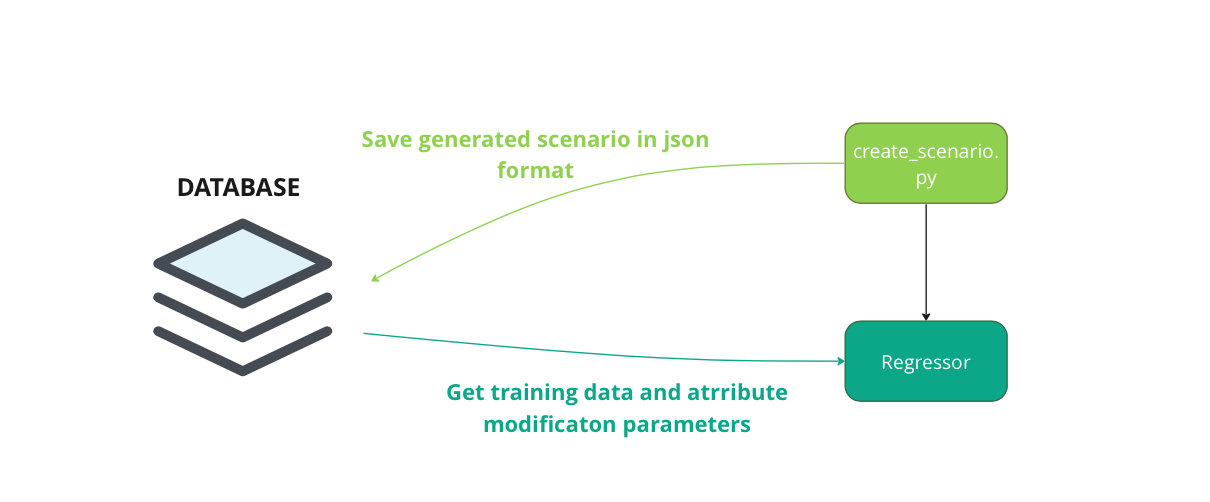
\includegraphics[width = 0.8\textwidth]{research_paper/Images/scenario_generation.png}
    \caption{Scenario generation overview}
    \label{fig:generation}
\end{figure}


One thing that was not mentioned yet is why the chosen labels are difficulty, wetness and sun altitude angle. The first one, difficulty, describes how complex the scenario is overall. For instance, the harsher the weather conditions and the more disobedient drivers there are, the more challenging the scenario is. The second label, wetness, is used to differentiate between dry and clear weather and rainy or stormy weather. The smaller the wetness value, the smaller the attribute values related to precipitation, fog, rain deposits, etc. The third and last label, the sun altitude angle, is used to differentiate between the different times of the day. To sum up, these three labels allow the algorithm to generate the scenario of desirable difficulty, wetness level and also the preferred time of day.

\section{Building paths and populating the simulator} \label{sect-5.3}

The previous section mentioned that the scenarios generated by the scenario generation algorithm are used by the PathBuilder and Scenario classes. Let us begin by discussing the path generation method this article proposes. 

To test how the vehicle is performing in the scenarios, it is not enough to specify the weather parameters or how many other participants will be involved. We need to give the vehicle an objective that it would try to achieve. In this case, the aim of the car is to drive some route and reach the destination safely.

Luckily, as this project aims to create a framework for automatic vehicle safety testing, manual path generation for every run is not a valid solution. That is why the PathBuilder class was developed (stored in  software/carla\_scripts/scenarios/path\_builder.py). This class is responsible for creating a path given the scenario JSON file.

The algorithm works as follows; first, it looks at all possible maps in the data/maps/opendrive\_format directory and loops through all the maps looking for one that satisfies the following criteria from the scenario file: 

\begin{equation} \label{requirements_for_map}
\begin{cases}
    number\_of\_junctions \le total\_number\_of\_unique\_junctions\_in\_map \\
    distance\_in\_metres \le total\_map\_road\_length
    \end{cases}
\end{equation}

If the map that is being analysed satisfies the criteria, it is chosen, and the path-building algorithm proceeds to try and create a path on that map; if the map does not meet the criteria or a path cannot be created in it, the algorithm takes another map and proceeds with the same actions until a path is generated or the algorithm is aborted meaning it is impossible to create a path in any of the maps given the scenario requirements.

It is also worth mentioning how the path itself is created when the correct map is found. If a valid map is found, the algorithm proceeds as follows: first, it selects a road element randomly, then enters a while loop and keeps looking for road successors, adding them to the list of checkpoints until the scenario criteria are satisfied. The successor elements can be of two types: a road element or a junction. If the currently analysed road element points to another road element, the while loop proceeds with the successor road element in the next iteration. However, if the current road element points to a junction, then a random successor of the junction is selected for the next iteration. Note that the successor of the junction is always a road element. If at any point the algorithm encounters a loop (two road elements pointing to each other) or a dead-end, it starts the process all over again. The algorithm currently has a limited amount of tries that it can have on a single map $x = 10,000$. If in $x$ tries the creation of the path is unsuccessful, the map file is either corrupt or a path there cannot be generated. This is made so that the algorithm never enters eternal while loops. The high level overview of the algorithm can be seen in the pseudocode fragment below:

\vspace*{1em}
\begin{algorithm}
\caption{High-abstraction-level path building algorithm}
  \begin{algorithmic}
    \Procedure{PathBuilding}{$scenario$} 
      \State $maps\gets \texttt{read OpenDrive maps from the database}$
        \For{$map\texttt{ in } maps$}
        \If{$map \texttt{ is valid}$}
            \State $r\gets \texttt{randomly pick a road element from the map}$
            \State $road\_elements \gets \texttt{[]}$
            \State $total\_length\gets 0$
            \State $number\_of\_junctions\gets 0$
            \While{$number\_of\_junctions < required\_number\_of\_junctions \newline
            \hspace*{10em}\texttt{ and } total\_length < required\_total\_length \newline
            \hspace*{10em}\texttt{ and not } road\_elements \texttt{ contains dead-ends}$}
                \State $total\_length \gets total\_length + r.length$
                \State $road\_elements.insert(r)$
                \State $successor \gets r.successor$
                \If{$successor$ \texttt{is junction}}
                    \State $number\_of\_junctions\gets number\_of\_junctions + 1$
                    \State $r \gets \texttt{random } successor \texttt{ exit that is not current } r$
                \EndIf
                \If{$successor$ \texttt{is road element}}
                    \State $r \gets successor$
                \EndIf
            \EndWhile\label{euclidendwhile}
            \State $path \gets \texttt{build path from } road\_elements$
            \If{$path$ \texttt{was found}}
                    \State \textbf{return} $path$\Comment{Else, try another map}
            \EndIf
        \EndIf
      \EndFor
      \State \textbf{return} $None$\Comment{If no path was found over all the maps, return None}
    \EndProcedure
  \end{algorithmic}
\end{algorithm}

If the maps in the opendrive\_format directory are well formatted, the final generated path could look like the one presented in \autoref{fig:good_path} where the blue colour marks the beginning and the red one the end. The colourful lines, gradually moving from blue to red, indicate the lanes that a vehicle can drive on. To draw the path on the map, the draw\_lanes\_terminal.py script has to be run with the path's name as the argument -p. The script is located in software/carla\_scripts/helper\_scripts directory.

\begin{figure}
    \centering
    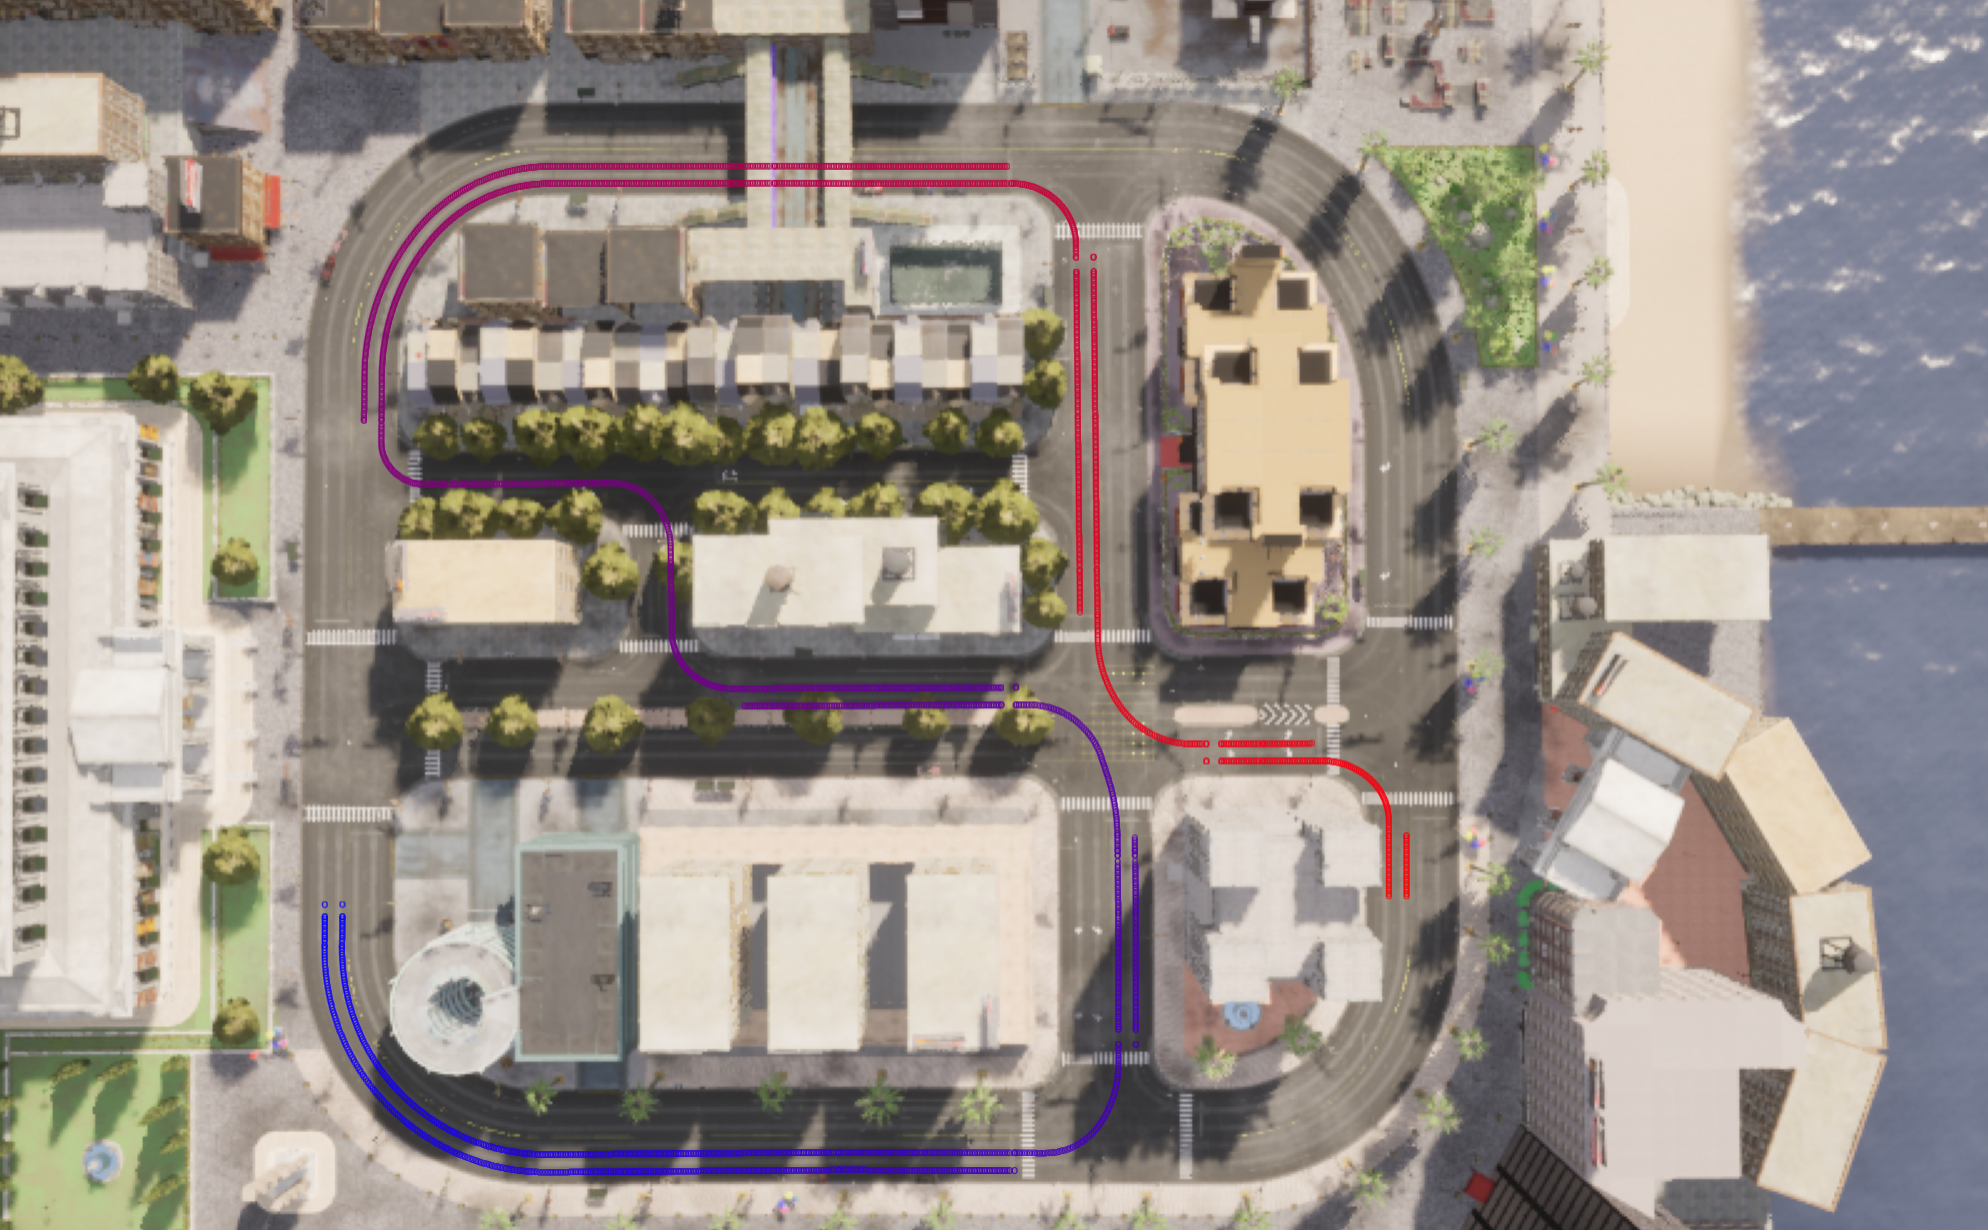
\includegraphics[width = 0.8\textwidth]{research_paper/Images/path1.png}
    \caption{Well-formatted path}
    \label{fig:good_path}
\end{figure}

However, the algorithm not always behaves in our best interest. In \autoref{sect-4.2}, when discussing the limitations of the simulator, we mentioned that CARLA is only as accurate and good working as the algorithms that power it. One of its issues revealed itself when designing this path generation algorithm. To begin with, CARLA, for its map specifications, uses OpenDRIVE format, which is a standard way of specifying map layouts and road networks\cite{dupuis2010opendrive}. The algorithm proposed by this article also uses OpenDRIVE files to analyse the road networks and thus generate paths.

As mentioned before, when a map is determined, the path generation algorithm randomly takes the first road element. If that initial pick is indeed a valid road segment, the algorithm can generate a path like the one pictured in the \autoref{fig:good_path}.

Unfortunately, the bigger part of OpenDRIVE maps provided by CARLA are poorly structured in some places (in version 0.9.13), meaning that the files specify that a road element is present when it is not. An example of a generated incorrect path can be seen in figure \autoref{fig:wrong_path}, where the points selected by the algorithm are outside the map where there is no road. After analysing the OpenDRIVE maps provided by CARLA, it was discovered that the specifications are indeed misleading. In addition, some maps possess other issues, like one road element pointing to itself or loops where two distinct road segments point to each other. The problems are illustrated in \autoref{fig:road_31} and \autoref{fig:road_41} in \autoref{chap:c}.

An example of a generated path can be found in \autoref{fig:generated_path} in \autoref{chap:a}. The points from the list \textbf{path\_checkpoints} are used by the GlobalRoutePlanner to build a path that a vehicle has to drive. The \textbf{town} attribute indicates the map, and the \textbf{start\_location} tells where to spawn the car.

\begin{figure}
    \centering
    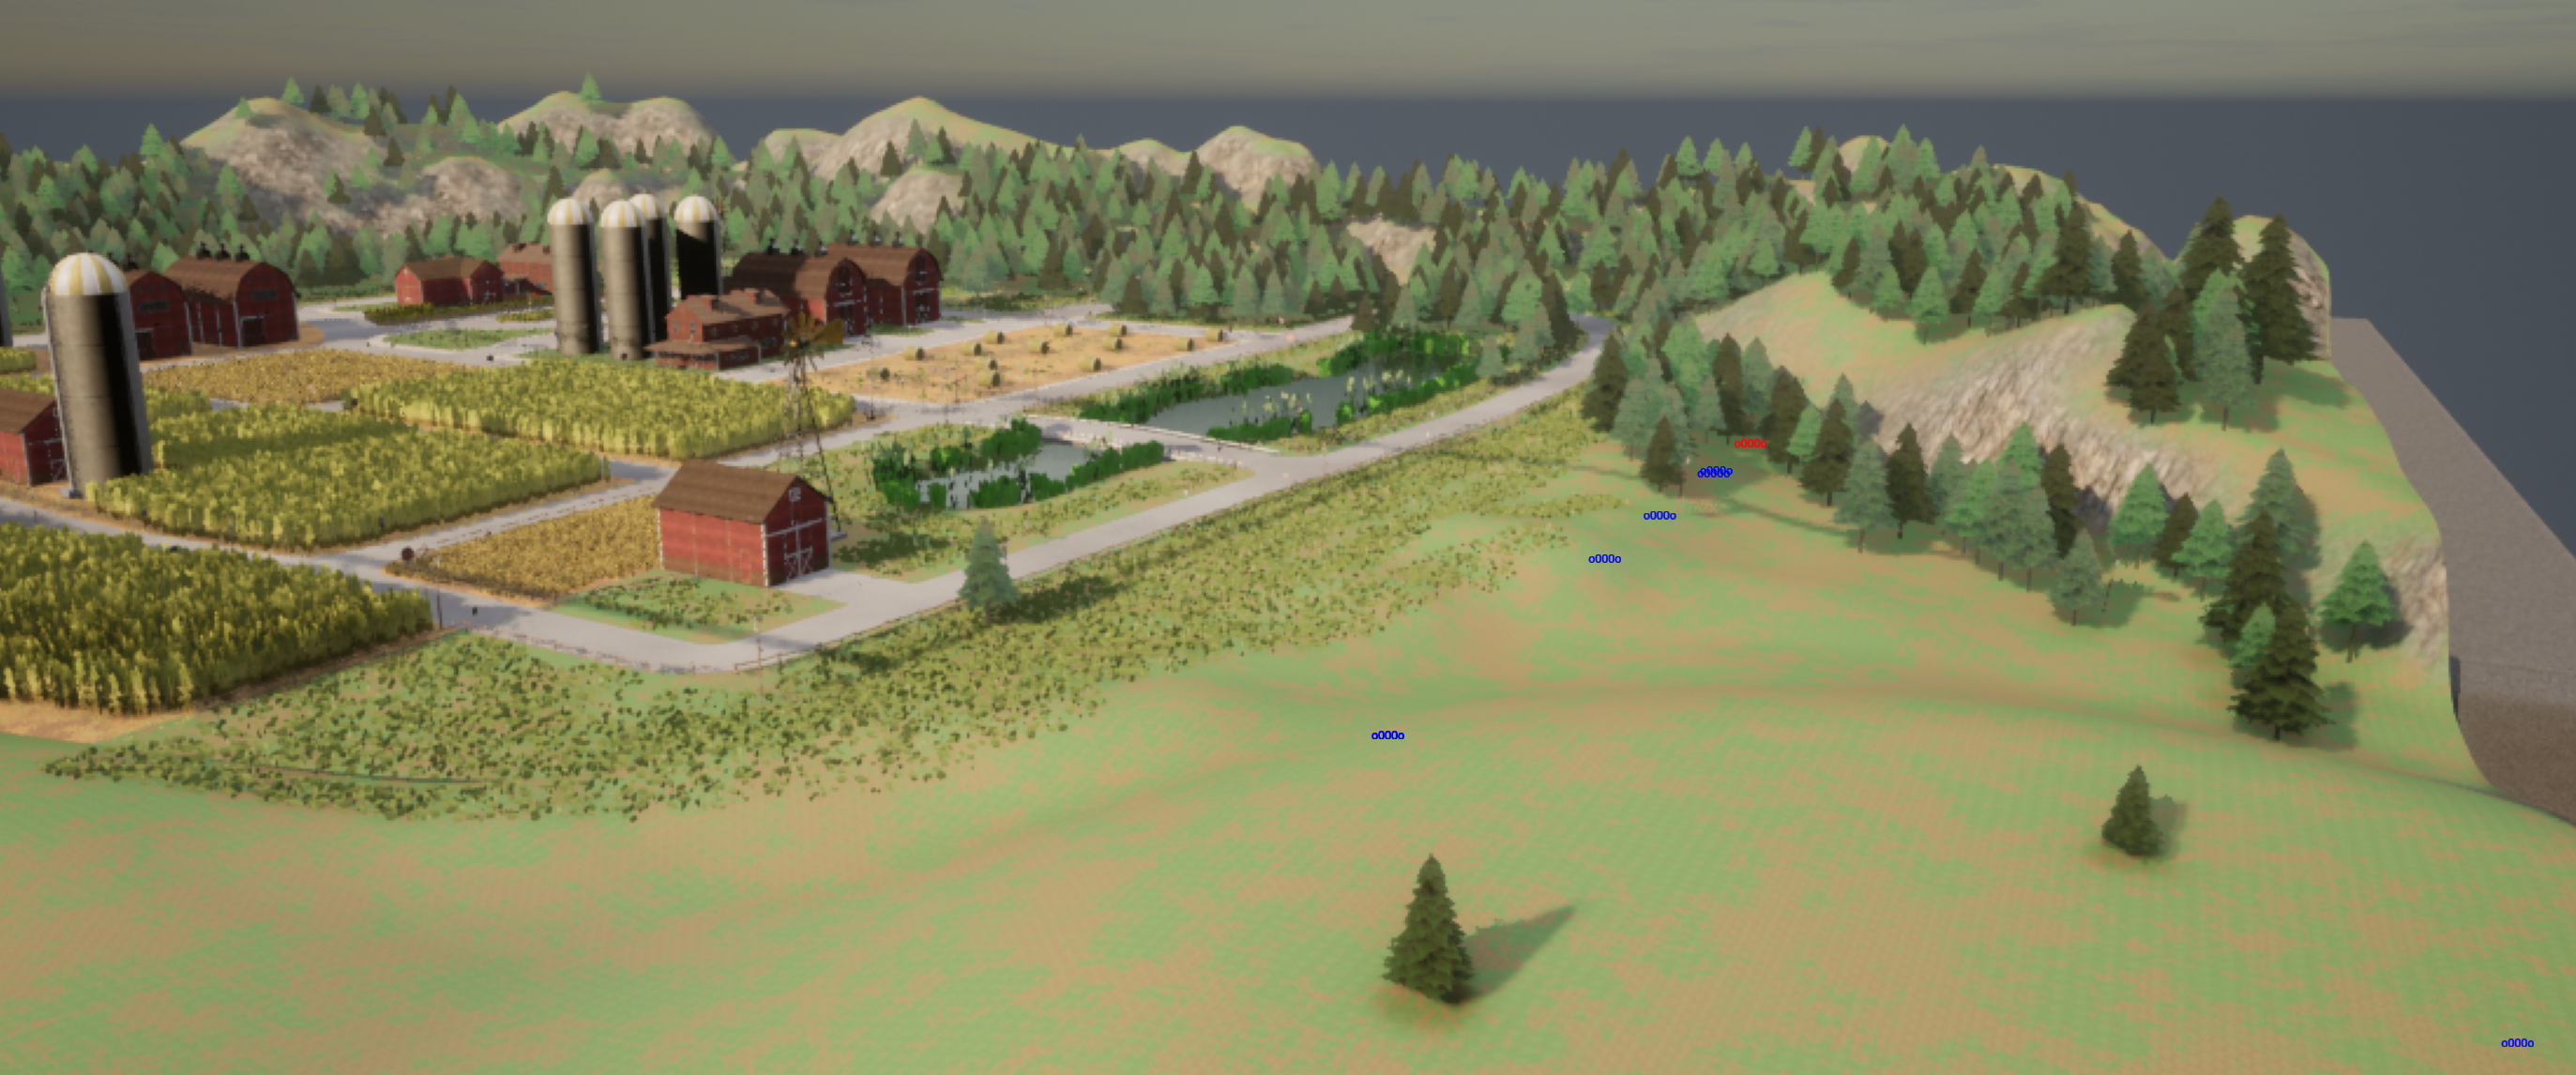
\includegraphics[width = 0.8\textwidth]{research_paper/Images/wrong_path.png}
    \caption{Poorly-formatted path}
    \label{fig:wrong_path}
\end{figure}

Now that we have talked about the PathBuilder and the issues it was facing, it is time to look at how the Scenario class uses both the generated path and the generated scenario to fulfill the simulation requirements. The Scenario class can be seen as a module responsible for spawning all the non-hero actors and specifying their behaviour according to the generated scenario attributes.

It first tries to spawn the necessary amounts of pedestrians, vehicles and two-wheel vehicles. If there are not enough spawn points for all the cars, the maximum number of them is spawned. After a successful spawn, the module customises the behaviour of all actors according to the values provided in the scenario file. For instance, if the $proportion\_of\_light\_ignoring\_vehicles = 0.2$ and the $light\_ignoring\_percent = 50$, then the algorithm randomly selects a fifth of the vehicles and sets their behaviour as such: when a red traffic light is approached, there is a 50\% chance that the car will ignore the traffic light. It does so, for all the behaviour-changing scenario attributes. Once the actors are spawned and their behaviour is set, the Scenario module assigns all the actors to TrafficManager to take care of their movements in the simulation. How the simulation takes place and when the TrafficManager is called will be discussed in more detail in \autoref{chap:eight}, when we talk about what the simulation session looks like and how all the components work together.

\section{Possible future improvements} \label{sect-5.4}

Having introduced the scenario generation methodology, it is now time to finish this chapter by discussing the possible improvements that could be implemented in the future.
First, to ensure that invalid paths are never generated, well-formatted OpenDRIVE map specifications should be used. From all the current map specifications, after some testing, only the Town01 showed the potential of being well-formed. Using other maps sometimes produced wrong paths.
Another part that should be improved is the path-building algorithm itself. Right now, it creates the paths by randomly trying to create one. It would be better if it did this in some structured way, looking for interesting patterns that could be utilised. However, the OpenDRIVE files currently contain only information about the road elements and junctions, providing very little extra information. In other words, more sophisticated road network descriptions should be used, providing information about roundabouts, highways, u-turns, road signs and other things.
Finally, the scenario generation algorithm could be improved in several ways. Firstly, well-described and realistic scenarios could be used for training. Currently, the algorithm uses naively generated training data, as discussed in \autoref{sect-5.2}. Furthermore, the machine-learning algorithm could be improved or even changed to use deep neural networks and predict scenarios from more sophisticated training data sources like video material.